\documentclass[tikz, border=10pt]{standalone}
\usepackage{xcolor}
\usepackage{fontspec}
\usepackage{tikz}

% Load TikZ libraries
\usetikzlibrary{
    positioning,     % For placing nodes relative to each other
    shapes.geometric,% For rounded rectangles
    arrows.meta,     % For custom arrowheads
    shadings,        % For gradient fills
    backgrounds      % To set a background color for the picture
}

% --- Define custom colors based on the image ---
\definecolor{BackgroundColor}{RGB}{241, 241, 250}
\definecolor{BorderColor}{RGB}{58, 74, 139}

% Define colors for gradients
\definecolor{gradBlue}{RGB}{196, 222, 246}
\definecolor{gradPurple}{RGB}{218, 203, 241}
\definecolor{gradYellow}{RGB}{253, 222, 160}
\definecolor{gradPink}{RGB}{240, 198, 223}
\definecolor{gradRed}{RGB}{255, 122, 142}
\definecolor{gradCyan}{RGB}{155, 230, 248}

% --- Define custom shadings for the gradient blocks ---
% Shading for 'Conv' blocks (Blue to Purple)
\pgfdeclarehorizontalshading{conv_shading}{100bp}{
  color(0bp)=(gradBlue);
  color(50bp)=(gradBlue);
  color(100bp)=(gradPurple)
}

% Shading for 'MaxPool2d' blocks (Yellow to Pink)
\pgfdeclarehorizontalshading{pool_shading}{100bp}{
  color(0bp)=(gradYellow);
  color(50bp)=(gradPink!80!gradYellow);
  color(100bp)=(gradPink)
}

% Shading for 'Concat' block (Cyan -> Purple -> Red)
\pgfdeclarehorizontalshading{concat_shading}{100bp}{
  color(0bp)=(gradCyan);
  color(50bp)=(gradPurple);
  color(100bp)=(gradRed)
}

\begin{document}

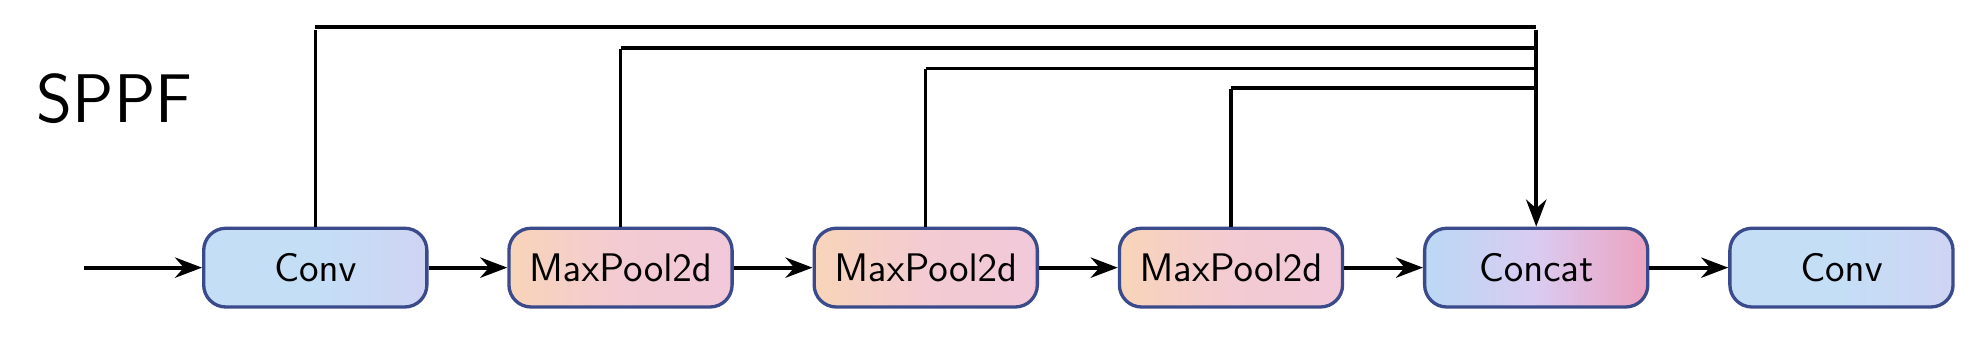
\begin{tikzpicture}[
    % Set a global font
    font=\sffamily,
    % Define a style for the blocks
    base_block/.style={
        draw=BorderColor,
        line width=1.2pt,
        rounded corners=8pt,
        minimum height=1cm,
        text width=2.6cm,
        align=center,
        font=\sffamily\Large
    },
    % Define styles for each gradient type, inheriting from base_block
    conv_block/.style={base_block, shading=conv_shading},
    pool_block/.style={base_block, shading=pool_shading},
    concat_block/.style={base_block, shading=concat_shading},
    % Define style for arrows
    arrow/.style={
        -Stealth,
        line width=1.5pt,
        black
    }
]

% Set the background color for the entire tikzpicture
% \begin{scope}[on background layer]
%     \fill[BackgroundColor] (current bounding box.south west) rectangle (current bounding box.north east);
% \end{scope}

% --- Place the nodes (blocks) ---
% Node names are chosen for clarity: c1, m1, m2, m3, cat, c2
\node[conv_block] (c1) {Conv};

% Place subsequent nodes to the right of the previous one
\node[pool_block, right=1cm of c1] (m1) {MaxPool2d};
\node[pool_block, right=1cm of m1] (m2) {MaxPool2d};
\node[pool_block, right=1cm of m2] (m3) {MaxPool2d};
\node[concat_block, right=1cm of m3] (cat) {Concat};
\node[conv_block, right=1cm of cat] (c2) {Conv};

% --- Draw the arrows between nodes ---
\draw[arrow] ([xshift=-1.5cm]c1.west) -- (c1.west); % Input arrow
\draw[arrow] (c1.east) -- (m1.west);
\draw[arrow] (m1.east) -- (m2.west);
\draw[arrow] (m2.east) -- (m3.west);
\draw[arrow] (m3.east) -- (cat.west);
\draw[arrow] (cat.east) -- (c2.west);

% --- Draw the SPPF label and skip connections ---
\node[font=\sffamily\Huge, above left=1.2cm and 0cm of c1] {SPPF};

% Define a coordinate for the horizontal path of the skip connections
\coordinate (skip_y) at ([yshift=2.5cm]c1.north);
\coordinate (skip_y1) at ([yshift=2.25cm]m1.north);
\coordinate (skip_y2) at ([yshift=2.0cm]m2.north);
\coordinate (skip_y3) at ([yshift=1.75cm]m3.north);

% Define coordinates for the "elbows" where vertical lines meet the horizontal path
\coordinate (c1_elbow) at (c1.north |- skip_y);
\coordinate (m1_elbow) at (m1.north |- skip_y1);
\coordinate (m2_elbow) at (m2.north |- skip_y2);
\coordinate (m3_elbow) at (m3.north |- skip_y3);
\coordinate (cat_elbow) at (cat.north |- skip_y);

\coordinate (cat_elbow_m1) at (cat.north |- skip_y1);
\coordinate (cat_elbow_m2) at (cat.north |- skip_y2);
\coordinate (cat_elbow_m3) at (cat.north |- skip_y3);


% Draw the vertical risers
\draw[line width=1.2pt] (c1.north) -- (c1_elbow);
\draw[line width=1.2pt] (m1.north) -- (m1_elbow);
\draw[line width=1.2pt] (m2.north) -- (m2_elbow);
\draw[line width=1.2pt] (m3.north) -- (m3_elbow);


% Draw the horizontal "triple line" bundle.
% We draw three lines, slightly offset, to create the visual effect.
\draw[line width=1.2pt, transform canvas={yshift=1pt}] (c1_elbow) -- (cat_elbow);

\draw[line width=1.2pt, transform canvas={yshift=0.5pt}] (m1_elbow) -- (cat_elbow_m1);

\draw[line width=1.2pt, transform canvas={yshift=0.25pt}] (m2_elbow) -- (cat_elbow_m2);

\draw[line width=1.2pt, transform canvas={yshift=0.25pt}] (m3_elbow) -- (cat_elbow_m3);


% Draw the final arrow from the bundle down to the Concat block
\draw[arrow] (cat_elbow) -- (cat.north);

\end{tikzpicture}
\end{document}